\chapter{Kappa}
\section{Introduction}

%On every continent there are hundreds of states that were until relatively recently
%independent and sovereign entities, much like the those who survived until
%today. Many, if not most, of them were amalgamated into larger states through
%the process of colonisation.\footnote{The two major exceptions are the
%unification of Germany and Italy.} 

In North West Indonesia, 1976, GAM (Gerkan Aceh Merdeka: Free Aceh Movement)
declared the independence of the province of Aceh under the leadership of Hasan
di Tiro, a descendent of the last Sultan of the Aceh region. Initially the
movement consisted of the remnants of an old religious network, with its roots
in the old Sultanate and armed struggle against the Dutch. The resulting
conflict lasted until 2005 and resulted in an estimated 3,402 combat related
fatalities after 1989 \citep{Aspinall2009, Pettersson2018, Sundberg2013}.

In Ethiopia in 1975, the Dirge regime tried to arrest the Sultan of Aussa. However,
anticipating the move, the Sultan's son had already sent men to neighboring
Somalia to train in guerilla warfare \citep{Shehim1985}. The Sultan evaded
arrest and launched the Afar Liberation Front (ALF) organized around the men
trained in Somalia. The heavy handed response of the Ethiopian military left
over a thousand civilian casualties \citep{UCDPconflict363}.

In 1960, in the newly formed Republic of the Congo (Léopoldville) (current
Democratic Republic of the Congo) South Kasai declared unilaterally to have
seceded from the nascent Republic under the leadership of traditional chief
Albert Kalonji \citep{Nzongola2002}. He then preceded to have his father
declared the new Mulopwe, thus resurrecting the royal title of the Luba kingdom
(1585-1889). His father promptly abdicated, handing the title to Kalonji (now
styling himself Albert Ditunga, `homeland'). South Kasai fought for independence
for just over two years, provoking a campaign by the Congolese armed forces that
at the time was characterized by UN Secretary-General Dag Hammarskjöld as an act
of genocide \citep{Nzongola2002}.

There is no shortage of examples where previously independent states are
involved in outbreaks of organized violence. Yet, both in the media and in the
academic literature these examples are referred to as ethnic conflicts, and
surprisingly little attention has been given to their connections to past
statehood. On the other hand, there are also examples of old state institutions
working for peace, mediation and reconciliation. For example, in Burkina Faso
the Mogho Naba of the Mossi kingdom of Ouagadougou served as a mediator
following a coup, and apparently was instrumental in preserving the peace
(\href{https://www.bbc.com/news/world-africa-34340704}{BBC}). [Another example
of peace inducing]. 

The nascent academic literature on organized violence and the legacies of past
statehood reflects these diverging sets of examples. While some, in line with
the examples given above, find a conflict inducing effect of past states
\citep{Englebert2002, Paine2019}, others argue that past experience of statehood
provides experience and institutions that are peace inducing \citep{Wig2016,
Wig2018, Depetris-Chauvin2016}. Yet, all but one of these articles conceptualize
states in terms of currently (politically relevant) ethnic groups and the degree
to which these groups have connections to past states. This risks excluding
states that are not readily tied to a current politically relevant ethnic group.
It further risks discounting experiences of statehood of groups who have lived
as a part of states for hundreds of years, without being the dominant ethnic
group. Additionally, this literature has been almost exclusively limited to
Africa. The diverging conclusions in the literature could in part be a result of
the paucity of quantitative data on past statehood. The literature has been
limited to using either the Murdoch map, which codes `jurisdictional hierarchy'
of ethnic groups, or the State Antiquities Index, which measures country level
experience of statehood (including from foreign rule). In summary, there is a
need for more and better data, in order to answer the puzzle of whether there is
a positive or negative association between state histories and organized
violence. Potentially, both statements are true, but vary according to
circumstances. In which case, what determines when and where past statehood is
conflict inducing or peace inducing?

%\textbf{What do I do to address the problem/puzzle?}

How is organized violence shaped by the underlying topography of historical
statehood? This thesis seeks to answer this overarching research question,
adding to our general understanding of organized violence. Increasing the
general understanding of concepts that matter to society, and attaining
knowledge in general, is an intrinsic goal of social science as a whole. The
hope that better understanding organized violence will contribute to conflict
prevention and de-escalation, is a further motivating factor for this thesis.
However small or insignificant the real world impact on these processes may be.

The main argument of the thesis is that historical states can have both conflict
inducing and conflict reducing effects depending on the type of conflict in
question\footnote{\label{note1}African sample.}, the number of historical state
entities contained within the boundaries of modern countries, and the distance
between where the pre-colonial state was present and the post-independence
capital\textsuperscript{\ref{note1}}. Specifically, when historical state
legacies are located far from the capital, they provide \textit{symbols of
sovereignty} that can be use to mobilize for violence, and \textit{local elite
networks} are often left behind and can mobilize their networks if their
interests are threatened by the government. While on the other hand, when
located near the capital, historical state legacies provide a foundation on
which modern states could be built. By providing legitimacy and institutions
such as an experienced security apparatus, pre-colonial states can significantly
limit violence when it breaks out in the capital.

The number of historical state legacies within a country matters because the
more of these there are, the more likely that one or more of them will be
located in a remote part of the country (and thus be conflict inducing).
Furthermore, increasing the number of potential claims making actors
incentivises the government to punish (engage in conflict) groups it would
otherwise accommodate in order to prevent other groups to make similar demands.

Just like the modern state has incentives to prevent its citizens from killing
each other and destroying each others property (such activities represent a dead
loss to tax income), historical states had the same incentives. As a
consequence, historical state legacies provide local institutions and traditions
of conflict resolution, as well as build up trust between communities, which
prevent outbreaks and escalation of communal violence. Where little or no
historical state legacies exist, and the modern state is weak or absent, groups
are limited to less effective mechanisms (such as intra group policing) to keep
the peace. In other words, when it comes to \textit{communal violence} there is
an inverse relationship between historical state legacies and organized
violence.

The thesis addresses the research question across four individual articles and
contribute to the literature through substantial data collection, and novel
theory building, which breaks new ground on a so far `under-researched' part of
the larger peace- and conflict research. The thesis has contributed to two data
projects. The Anatomy of Resistance Campaigns (ARC) and the Geo-International
Systems Data (Geo-ISD). The ARC project collected yearly data on 1,426 organizations
engaging in maximalist dissent (non-violent and violent) in Africa from 1990 to
2015. The Geo-ISD geocodes the borders of independent states in Africa from
1800 to 1900, which are used to generate a measure of their respective
historical presence per 0.5 X 0.5 degrees grid cell. 

In summary, the thesis finds that the historical legacies of statehood's
relation to organized violence depends on:\\

1) Distance to capital. In paper 3 I find that more pre-colonial state presence
is conflict inducing far from modern capitals, but conflict reducing when
close.\\

2) The number of historical states within modern a modern states. In paper 2 we
find that having more distinct historical state legacies is conflict inducing on
the state level.\\

3) Type of organized violence. While both paper 2 and 3 find conflict inducing
effects of historical state legacies on civil conflict, paper 4 finds that the
relationship to communal violence is the other way around. Paper 4 finds that
the stronger the presence of pre-colonial states, the less communal violence an
area experienced in the post-cold war period.

\section{Existing literature} \label{Existing literature}

\subsection{Correlates of civil war and non-state conflicts} 
\label{Correlates of civil war and non-state conflicts}

Studies of civil conflict have found a number of correlates,\footnote{As opposed
to \textit{causes}, which will be discussed in Section \ref{Models}.} some more robust
than others. While democratization itself may be a violent process, intermediate
regimes are most prone to civil conflict of all regime types, stable democracies
are the least prone to such violence \citep{Hegre2001, Goldstone_2010}. 
Oil and natural resource wealth, has been found to increase the likelihood of
conflict onset and on the duration of conflict \citep{Lujala2010, Lujala2005,
Lujala_2008, Ross_2006}. As opposed to various measures of ethnic diversity,
such as fractionalization, excluding ethnic groups from power reliably predicts
conflict \citep{CedermanLars-Erik2013Igac}. As does rough and mountainous
terrain \citep{Buhaug_2010, Hegre2006}.

Although the causal mechanisms underlying the relationship remains hotly debated,
the negative association between economic development and civil conflict is the
most consistent finding of all in civil conflict studies. Poverty itself
\citep{Hegre2006}, slow growth \citep{Hegre2006} and negative income shocks have
all been linked to increased risk of conflict.

Relative to the civil conflict literature the literature on non-state violence
is still in its infancy. Nevertheless, works have examined subjects ranging from
electoral violence \citep{Fjelde_2020, Salehyan_2014, Burchard_2015}, to rebel
on rebel violence \citep{Fjelde_2012, Lilja_2011, Cunningham_2012, Nygard_2014}
and refugees \citep{Bohmelt_2018}. More closely relate to this thesis is the
literature that has examined communal violence.

The quantitative literature on communal conflicts has focused on structural
causes that makes conflict more likely to trigger. In particular climate and
environmental factors have been shown to increase rates of communal violence
\citep{Turner_2011}. Both negative \citep{Detges_2017, Fjelde2012,
van_Weezel_2019, Petrova_2022} and positive \citep{Theisen2012, Witsenburg2012}
shocks to precipitation, have been shown to trigger communal violence. Others
have pointed to socioeconomic inequality \citep{Fjelde2014, PETERS_2004}, mixed
legal systems \citep{Eck2014}, marginalisation and corruption
\citep{BENJAMINSEN_2009} or state-building on pastoral lands
\citep{hagmann2008pastoral}.

\subsection{Historical legacies} \label{Historical legacies}

The literature on the long term effects of past statehood can broadly be
separated into the economic, political, and conflict outcomes, which I will
briefly summarise below.

\subsubsection{Economic legacies} \label{Economic legacies}

There is a growing literature demonstrating how historical states and
institutions still have lasting legacies today. Most of this literature has
examined the effects of past statehood \citep{Bockstette2002, Borcan2018} and
institutions related to statehood \citep{Michalopoulos2013, Michalopoulos2018,
Englebert2000} and largely agree on a positive effect of statehood and
institutions \citep{Nunn_2020, Michalopoulos2016} on long term economic
development. However, \citet{Acemoglu_2002} argues that European colonialism
lead to a `reversal  of fortunes' for the areas it affected. Poorer areas with
less population density (areas less likely to be at the center of states), were
less likely to be colonised early, `deeply', and with European settlers (in part
because of states more effectively resisting colonization). This lead to a
larger transfer of European institutional innovations, and consequently a
reversal of economic development \citep{Acemoglu_2002}. In an explicit attempt
to synthesize the `reversal' and `persistence' of fortunes, \citep{Foa_2017}
argues that the reversal of fortunes is subject to a threshold condition.
The most developed states were able to resist colonization (China, Japan and
Turkey), and instead engage in defensive modernization (adopting western
political innovations and technology). Those just below the threshold suffered
most at the hands of the colonizers, but have also seen the greatest
post-independence rebound, both in political and economic terms \citep{Foa_2017}.

%\citet{Grosjean_2011} finds that Ottoman rule
%suppressed financial development in Eastern Europe.

In large parts of Africa the Tsetse fly carries parasites that kill humans,
horses and cattle. This has caused lower population densities and difficulties
with state building, which in turn has translated to lower economic activity
today (as measured by night light density) in affected areas \citep{Alsan_2015}.

\subsubsection{Political legacies} \label{Political legacies}

A different branch of research has examined political implications of state
legacies. Building on \citet{Acemoglu_2002} , \citet{Hariri2012} test parts of
the proposed mechanism and finds that more pre-colonial experience of statehood
decreased the likelihood of being colonised, while it increased the likelihood
of only being \textit{indirectly} colonised. Furthermore, not being colonised,
or being so indirectly, depresses post-colonial democracy \citep{Hariri2012}.
\citet{Chlouba_2021} finds that exposure to early state development
(pre-colonial) is associated with support for autocratic rule in Africa.

On the other hand, through a number of case studies Wilfahrt
\citeyear{Wilfahrt2018, Wilfahrt_2021} has documented how areas and groups with
pre-colonial experiences of statehood are better at distributing public goods
equitably and efficiently, and are generally more likely to adopt non-group
based legislation and politics. The actors themselves ascribe this to their
history of cooperation (under the umbrella of pre-colonial states). This is even
true in Senegal, the poster child of French direct rule and dismantling of
pre-existing institutions \citep{Wilfahrt_2021}. Supporting earlier works of
\citet{Gennaioli_2007, Gennaioli2007a}.

\subsubsection{Legacies of violence and contention} 
\label{Legacies of violence and contention}

Living up to the second part of the quote attributed to Charles Tilly, `War
made the state, and the state made war.', past states can leave legacies of
conflict. Historical levels conflict in Africa have been found to positively
affect modern levels of conflict \citep{Besley2014}, although the direction of
the relationship is does not hold in a global sample, and depends on colonial
experiences and wars of colonial liberation \citep{Fearon2014}. 

%\citet{Dincecco_2019}

Similar to \citet{Clapham1996}'s notion of limited statehood, another branch of
literature has emphasized how African boundaries reflected colonial competition
between European powers, rather than the local ethnic, geographic or political
situation. For example, \citet{Alesina2011} uses `squigglyness' of international
boundaries as a measure/instrument for whether the boundaries were drawn with
local knowledge (endogenously), or not (exogenously). They find that
straightness of international boundaries, what they term artificial borders, are
linked with lower levels of economic development. The presumed mechanism (which
is not tested) is that artificial borders, borders drawn by an exogenous
process, group together multiple ethnic groups and split others. These ethnic
constellations then make it difficult for the state to create a sense of
nationhood and get people to work toward common goals. \citet{Englebert2002}
tests this more explicitly and find that states whose borders split ethnic
groups more, are more often involved in international disputes. They also find
that countries whose boundaries group together ethnic groups with more different
forms pre-colonial political organization\footnote{As measured by the standard
deviation of \citet{Murdock1967}'s jurisdictional hierarchy index.}, are more
susceptible to civil wars, political instability and secession attempts.
Following \citet{Englebert2002} the conflict-literature has also uncovered links
between ethnic partitioning and civil conflict \citep{Ito2020,
Michalopoulos2016}, as well as links between resulting trans-border ethnic kin
relations and conflict \citep{Cederman2013, Salehyan2009, Weidmann2015}. 

A handful of recent studies have examined how legacies of statehood can shape
violence and contention even to this day. \citet{Wig2016} finds that African
ethnic groups with more centralized pre-colonial institutions are less likely to
be involved in ethnic conflicts. He argues that many of these institutions are
persistent, and that institutions reduce commitment problems by reducing
uncertainty and imposing constraints on leaders \citep{Wig2016}. Similarly,
\citet{Depetris-Chauvin2016} finds that areas with more long run exposure to
statehood have experienced fewer years of post-cold war conflict (of any type
coded by the GED). He attributes this to better equipped with mechanisms to
establish and preserve order, and supports this by showing that individuals in
countries with more state history are more favorable to state institutions and
traditional leaders, and that such ares are more resistant to the conflict
inducing effect of negative economic shocks \citep{Depetris-Chauvin2016}.

On the other hand, \citet{Paine2019} examined ethnic groups in Africa organized
as pre-colonial states (PCS-groups), and how relate to non-PCS-Groups. He finds
that PCS-groups are likely to be in power, and that while in power they tend to
exclude other ethnic groups, increasing the risk of internal coups and civil
conflict from other groups \citep{Paine2019}. Overall, he finds that non-PCS
groups in countries with a PCS-group participated in major civil wars 4.9 times
more frequently than non-PSC-groups in countries without a PCS-group. Indeed, of
the thirty-two ethnic group-level major civil war onsets after 1989, thirty
occurred in countries with a PCS-group.

Studying communal conflicts \citet{Wig2018} employ bargaining theory from state
based conflict studies to demonstrate that institutions (like ones stemming form
former statehood) can provide credible non-violent bargains between groups. They
find that the more institutions an ethnic group has, the better it is able to
avoid conflict. They also find a conflict reducing effect of more inclusive,
democracy-like, institutions \citep{Wig2018}.

\subsection{Moving beyond the literature} \label{Moving beyond}

% Pain does not directly contradict DP and Wig, but does present a puzzle.
% Especially coupled with the artificial states literature.

As is evident from the introduction and the previous paragraph, there is
considerable ambiguity as to whether legacies of historical statehood have a
positive or negative impacts. Whether the outcome variable is long term economic
development, chances for democracy, public goods provision, or levels of
conflict and violence. This thesis seeks to address part of this puzzle, by
examining the relationship between state legacies and organized violence. The
thesis adds to the literature by showing that \citet{multiple} distinct state
legacies within the same country is one, previously overlooked, causal pathway
(Paper \ref{CB}). While Paper \ref{main} identify novel ways through which
pre-colonial states in Africa can be both conflict inducing as well as conflict
reducing. Finally, Paper \ref{OMT} establishes that the conflict
inducing/reducing effect of pre-colonial states in Africa further depends on the
type of conflict in question. Namely, that for communal violence the overall
effect of pre-colonial statehood is conflict reducing.

Additionally, the thesis addresses some of the shortcomings of the existing
literature by providing innovative new data on pre-colonial states (see Section
\ref{Analytical approach}), and using existing data in new ways.

\section{Concepts} \label{Concepts}
% Concepts and literature

\subsection{States} \label{States}

At the core of the thesis lies the concept of `the state'. However, the term is
ambiguous. Three of the four individual articles in the thesis use a specific
operationalisation, derived from \citet{Butcher2019} and \citet{Butcher2017},
but the concept merits further discussion than what the article format allows.
The subject of the thesis requires a definition that is broad enough to include
African and Asian states in the nineteenth century and modern European states.
It needs to be flexible to the changes in how we think of the state across time
(even in Europe, states were very different from today), as well as across
space. While at the same time it needs to draw the line at some point to say
what is not a state. To this end the thesis employs \citet{Clapham1996}'s three
aspect of the state, which allows assessing degrees of statehood along three
axes.

The first aspect of the state is the \textit{administrative}. The ideal of
which is an organization (government) which exercises sovereign jurisdiction
(the final legal arbiter) over a given population and territory. To exercise
this sovereignty the government controls a coercive apparatus (military and
police forces), which is usually financed by taxing the population. In return,
modern states are usually expected to ensure the welfare of its
citizens/population (externalities, health, security, education etc.). A state
in this sense may be more or less able to control its population, and more or
less able/willing to provide welfare.

The second aspect of the state is the `idea of the state', as constructed in the
minds of at least those who run it, but usually also a portion of the population
living within a state. This construction provides legitimacy for its
institutions and its use of coercive force (governmental legitimacy), and for
who, or where it should rule (territorial legitimacy). Today most states draw
their governmental legitimacy, their right to rule, from claiming (more or less
truthfully) to rule on behalf its citizens through democratic
principles.\footnote{Even the most blatant autocracies make this claim
\citep{FukuyamaFrancis2014POaP}.} Historically, various forms of religious
justification have been the norm (divine right of kings in Europe, the mandate
of Heaven in China, or rulers claiming to be gods or dependents of gods
themselves). Claims to territorial legitimacy (or lack thereof) usually rests on
a mix of historical precedence and the principle of national self determination.
Past claims include, rights to inheritance, religiously based rights to world
conquest, or the infamous `white mans burden'. The `idea of the state' and
legitimacy is key to ensuring compliance with minimal use (or threat) of
coercion \citep{BuzanBarry2007PSaF}. 

The third aspect of the state is the system of international recognition,
wherein states recognise each other, and respect (or even protect) each others
sovereign territories. In the current globalized world, international
recognition has become essential to participate in international transactions.
States that are lacking in the first and second aspects of statehood can lean
more on the international system, through aid (both from other states but also
non-state actors) and ideology. Prior to the twentieth century, multiple
international state systems existed. Even as late as the nineteenth century what
mattered to most Muslim rulers was recognition by the Caliph in Istanbul, not
what the kings or queens of Europe considered had to say on the matter.
Similarly in East Asia, China (the Middle Kingdom) was at the center of its
tributary-based international system, while South East Asia was organized in the
Mandala state system \citep{Hui_2005, KangDavidC2010EAbt}.

States can conform to each of these three aspects to a greater or lesser extent.
In other words, states have an overall degree of statehood, but also a
qualitative variation in terms of the individual aspects. Poor performance in
one aspect can be compensated, but only in part by strong performance in other.
Taiwan for example, has a robust and well functioning state apparatus, and is de
facto in undisputed control of its territory, enjoys a high degree of legitimacy
and compliance among its citizens, but struggles with a lack of full
international recognition. Israel has a high degree of administrative statehood, and
enjoys recognition from the most relevant actors (the exception being several
Muslim majority countries), but is viewed as largely illegitimate among many of
its Palestinian population, who represents roughly 20\% of its population.
Somalia (and other so-called `failed states') fare poorly across all three
aspects of statehood. The Somali government barely functions in and around the
capital, let alone the rest of its sovereign territory. Its government is
viewed as corrupt and illegitimate. Its borders do not reflect the settlement of
the Somali ethnic group, lacks any historic president, and are the product of
exogenous factors (external diplomatic negotiations). What little claim to
statehood Somalia has rests almost exclusively on the international system.

\citet{Clapham1996}'s argument is that post-independence Africa represents a new
model of statehood, where statehood rested almost exclusively on the
international system. They were in large part created by (large and important
wars of liberation/de-colonization notwithstanding) and eventually sustained by
the international system. At the very least their \textit{extent} was. This
amounted to a novel form of limited, or artificial statehood. I argue that this
process is not unique to Africa. In Asia too, Europeans created colonial states,
and left countries with limited degrees of administrative statehood and vague
`ideas of state'.

\subsubsection{Historical state entities and pre-colonial states} 
\label{Historical state entities and Pre-colonial states}

At this point a further clarification of the terms `past states', `pre-colonial
states', and `historical state entities' (the term used in the second article of
the thesis) is needed, as I have used these terms more or less interchangeably
in this [introductory chapter/narrative]. The reason they are used
interchangeably is that they do refer to the same \textit{concept}. However,
they apply to different \textit{contexts}. Specifically, I use `pre-colonial
states' in the context of Africa, where the majority of states were at some
point colonized. The other two terms are used in the global context and refers
to states that now form parts of sovereign states. The term `Historical state
entities' refers to the operationalisation used in the second article of the
thesis, which is further restricted to the time period of (1816-1939).

\subsection{Maximalist dissent and organized violence}
\label{Maximalist dissent and organized violence}

Another key concept of the thesis is collective action; people cooperating in a
more or less organised fashion, to a achieve more or less common goals.
Organizing in such a way is harder than it might seem.
\citet{OlsonMancur1965TLoC} and \citet{Tullock_1971} emphasise the difficulty of
overcoming the barriers to collective violent action and the free rider problem.
For example, organizing to overthrow a despised dictator involves substantial
risks, while the benefit for successfully overthrowing him befalls equally to
everyone, regardless of participation. In particular, this thesis is concerned
with two partially overlapping forms of collective action, namely
\textit{maximalist dissent} and \textit{organized violence}. Figure \ref{venn}
illustrates how these forms of collective action relate to each other, and the
following discussion will provide more details.

\begin{figure}[htpb]
	\centering
	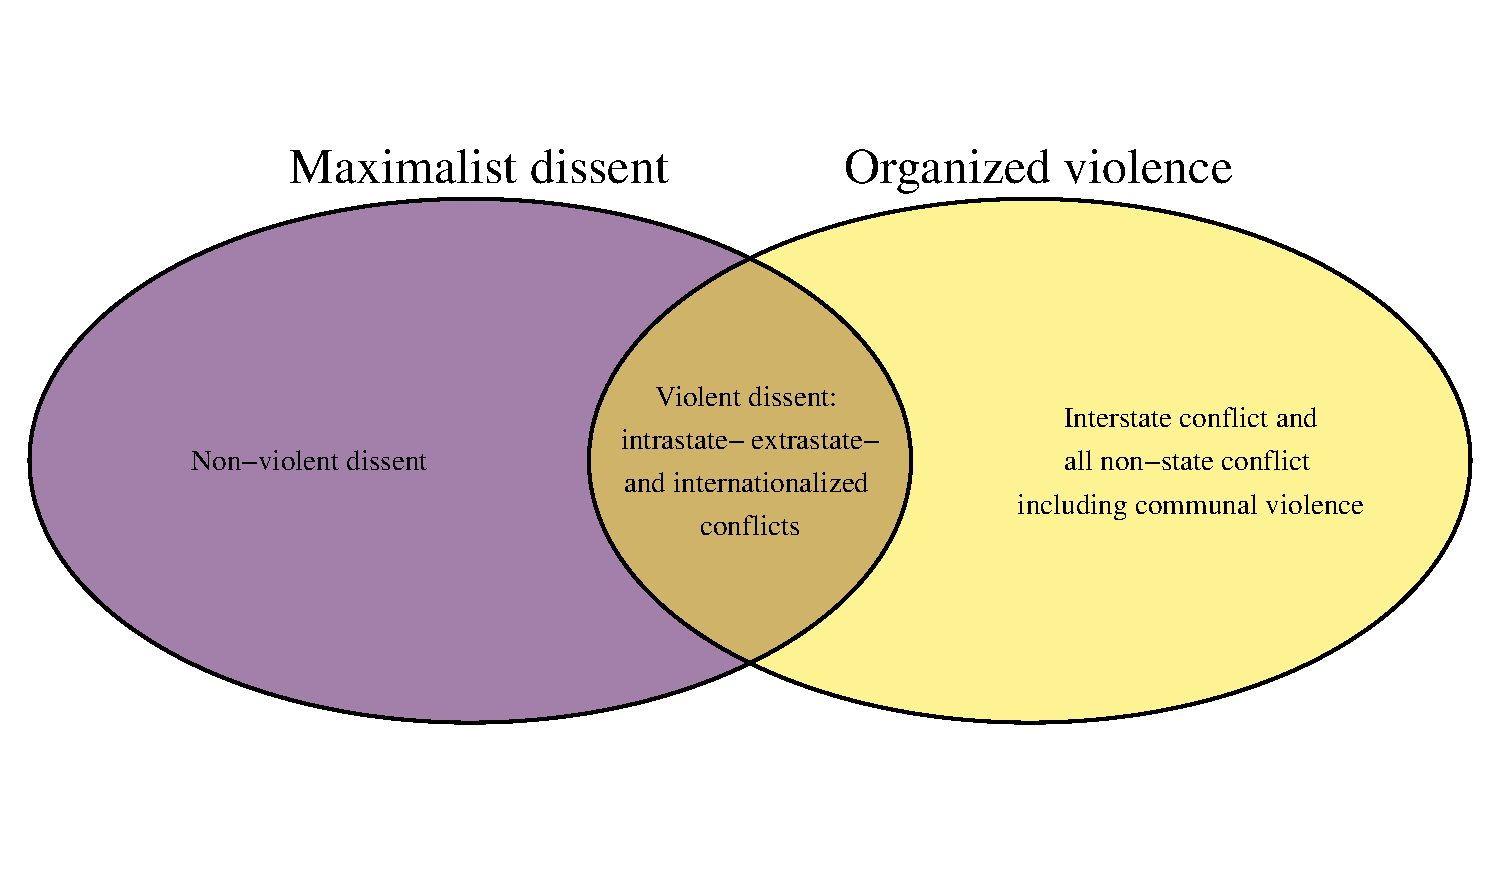
\includegraphics[width=\textwidth]{../R/Output/venn.pdf}
	\caption{Categories of violence and dissent}
	\label{venn}
\end{figure}

\subsubsection{Maximalist dissent} \label{Maximalist dissent}

[Given its relatively lesser importance I think it is OK to keep the literature
discussion here, rather than to separate this section into tow tiny sections
(here and in the correlates section)]

%Tarrow 1998, `power in movement is cumulative'

A central concept in the first article of the thesis is maximalist dissent. The
concept builds on \citet{TillyCharles1978Fmtr}'s definition of collective
dissent as observable action involving multiple people, beyond normal
institutional procedures for realizing political goals. This could include
anything from strikes, sit-ins, shirking, large scale demonstrations and other
non-violent tactics, to riots, terrorism or armed rebellion. It does not include
acts of dissent executed in an individual capacity, acts that lack clear
political goals and acts within institutional political bounds (regular
functioning of political parties, lobbying, electoral participation etc.). The
second part of the concept, maximalist, refers to the political goals of the act
(event). The definition builds on the criteria used by the NAVCO 1 data set,
which only includes resistance campaigns where the objective was maximalist
(i.e. regime change, secession, or self-determination) as opposed to limited
(i.e. greater civil liberties or economic rights)
\citep{DVN/0UZOTX/B4RH7S_2019}. The ARC data (presented in article 1) clarifies
this further as demands that calls for changes in the political structure that
would significantly alter the executive’s access to state power, the rules with
which executives are selected, or the policy or geographic areas for which the
executive has the right to make laws \citep{Butcher_2022}.

While the remaining articles of the thesis are concerned with organized
violence, most of which represent the violent part of the spectrum of maximalist
dissent (more on this below), the literature on the non-violent form of dissent
has informed the thesis in a number of ways as well. Understanding how, and
when, nonviolent forms of dissent work and when they do not, can help us
understand when and why people choose to pick up arms and use violence. Several
studies find that nonviolent dissent (or resistance) is the most effective of
achieving maximalist political goals \citep{chenoweth2011civil, Stephan_2008}
such as regime change and democratization \citep{Celestino_2013, Bethke_2019}.
Why then do some actors still chose violence? Part of the answer could be the
size of the target audience \citep{Gleditsch_2021}. Mass mobilization is
necessary for nonviolence to be successful. Goals that benefit a large part of
the population, such as overthrowing an unpopular autocratic regime, facilitate
mass mobilization. In comparison, groups who appeal to more narrow bases such,
as self determination for an ethnic minority, find mass mobilization difficult.
For such groups then, non-violence may not be effective, and so they pursue
their goals by violent means instead \citep{Gleditsch_2021}. Economic structures
could matter as well \citep{Butcher_2014}. A substantial literature is also
arguing that repression of nonviolent campaigns or protests, can cause
escalations to violence, although there is conflicting evidence
\citep{Chenoweth_2017, Lichbach_1987}.

Furthermore, a key reason for employing the term maximalist dissent is that
there is no sharp dividing line between violent and nonviolent forms of dissent.
In her study of the civil war in El Salvador \citet{Wood2003} highlights how
rebel groups cooperate and work closely with civil society, and how individual
rebels shift between violent and nonviolent forms of dissent. Many predominantly
nonviolent movements have violent wings, who increase the likelihood of
violent escalation -- especially if the nonviolent campaign fails to make
progress \citep{Ryckman_2019}.

\subsubsection{Organized violence}
\label{Organized violence}

There are many forms of organized violence, most of which are captured by
maximalist dissent. I follow the Uppsala Conflict Data Program (hereafter UCDP)
and \citet{Melander_2016} in treating organized violence as the aggregation of
the mutually exclusive typologies of one-sided, non-state and state-based
violence. One-sided violence is violence committed by formally organised
non-state groups or governments against unarmed civilians. State based is what
one usually thinks of as armed conflict, or simply war. More accurately, it is
armed conflict where at least one side is a government (and the other is not
unarmed civilians). This includes inter state conflicts (conflict between
states), extrastate conflict (decolonization-conflicts), intrastate conflicts
(conflicts within states, i.e. civil conflicts) and internationalised internal
conflicts (intrastate conflicts in which at least one party receives troops from
another state). Non-state violence is violence perpetrated by named
organizations (criminal organizations, political parties, rebel groups etc.) or
identity groups (ethnic or religious groups), against one another (without the
involvement of government). Non-state violence therefore is seldom driven
maximalist dissent, although clashes between political parties or politicised
ethnic groups could be potential borderline cases.

This thesis focuses on three forms of organized violence: intrastate,
internationalised internal conflict (hereafter referred to collectively as civil
conflict) and communal violence.\footnote{Historical state entities could matter
	for interstate conflict. For instance in cases where the borders of
	historical state entities cross international boundaries, old borders
	could form the basis of claims making and disputes, such as with the
	borders of the former empire of Bornu \citep{Hariri2012}. However, as in
	the case of Bornu, such disputes can be solved peacefully in
	international courts. Additionally, three of the four papers rely on an
	African sample and the continent have seen only one interstate conflict
and no extrastate conflicts in the time period covered in the papers.} 

Communal violence is organized lethal violence between identity groups. These
groups can identify along tribal, national, clan, religious, ethnic lines, or
any other source of identity, but are not permanently organized for combat, in
other words not rebel groups, formally organized militias or state coercive
apparatus. A key difference between communal conflicts and civil conflicts is
that both parties are, at least nominally/in a de jure sense\footnote{Gray
        areas include areas outside de facto state control, or cases where one
side acts with government impunity or backing.}, subject to the higher
authority of the government. For further discussion of the concept of communal
conflict see \citet{BroscheJohan2012Cccw}. While events that trigger such
conflicts can be often be relatively minor (theft, trespassing, illegal
grazing etc.) this type of violence tends to quickly spiral through reprisals
and counter reprisals and can rack up large death tolls and often far larger
displacement \citep{Horowitz_2001}. 

\section{Theoretical framework}
\label{Theoretical framework}

\subsection{Models} \label{Models}

There is a substantial literature explaining the occurrence (and re-occurrence)
of civil conflict. I broadly divide this literature into three overarching
[models/frameworks] that continue to influence not only the works presented in
this thesis, but in most of the academic literature on civil conflict. This
literature can be traced back to a handful of classic studies in the 1960s and
1970s. \citet{GurrTedRobert1970Wmr}'s theory of relative deprivation and the
related `revolution of rising expectations' \citep{Davies_1962} focused on how
widespread individual discontent laid the ground for revolution (Section
\ref{Grievance}. This \textit{grievance} model of civil conflict was met with
critique from the likes of Charles Tilly and  others, who instead argued that
rebellion happened when there were opportunities for it (Section
\ref{Opportunities}). A more recent branch of the literature build on models
from economic via international relations theory. Starting from the assumption
that both parties are (usually) best served with a non-violent bargained
solution, these models focus on the situations in which bargaining none the less
breaks down, or the exception when conflict becomes a rational choice (Section
\ref{Bargaining}).

\subsubsection{Grievance} \label{Grievance}

The grievance and deprivation focus of \citet{GurrTedRobert1970Wmr} and
\citet{Davies_1962} was later expanded on to include structural inequalities as
well \citep{Muller_1985, Muller_1987, ScottJamesC1977TMEo}. 

Responding to the criticism of the opportunities model, another branch of the
grievance literature shifted the focus to group level mechanisms,
moving away from strict Marxist or materialist explanations at class or country
level. For example, \citet{Hechter_1978} argued there was a cultural division of
labor, and that civil conflict occurred when cultural and economic groups
coincide. Others emphasized competition between ethnic groups for scarce
resources \citep{barth1969}. \citet{Horowitz1985}'s case studies demonstrated
how ethnic groups can garner intense feelings of belonging, collective
self-esteem and group worth, and that ethnic conflict was not just competition
for scares resources, but \textit{also} for political influence. He anticipated
the literature on horizontal inequality by stressing the role of cognitive
comparisons between groups as a mechanism for ethnic conflict. Despite the scale
of Horowitz's study, there was still a lack systematic empirical support for the
idea that grievances (group level or not) could lead to civil conflict. The
drive to address this gap was lead by Gurr and the minorities at risk (MAR)
project \citet{GurrTedRobert1993Mar:}. In response to Tilly's earlier
critique he also added some opportunity to the general argument of grievance in
the resulting work \citep{Gurr_1993}. 

In response to the lack of explanatory power of commonly used measures in the
quantitative literature on ethnicity and civil conflict like ethnic
fractionalization \citep{Alesina2003, Posner2004} and polarisation
\citep{Montalvo2005}, a more recent branch of the grievance literature has
turned to radical disaggregation in an effort to tighten the logic of causal
inference. This literature has examined  the role of interpersonal grudges and
local score settling in civil violence \citep{Kalyvas2006, Kalyvas_2008}, as
well as the role of moral outrage at government injustice and a sense of doing
the right thing \citep{Wood2003}. Reflecting earlier work by \citet{barth1969},
others who expressed scepticism of how ethnic identities were used as analytical
units in civil conflict research, they argued that ethnic defection is more
common than previously assumed \citep{Kalyvas_2008, Staniland_2012}, and that
ethnic identities are essentially undetectable or too fluid be of analytical use
\citep{Gilley_2004, Chandra2006}. What is more, the state is not ethnically
neutral \citep{CedermanLars-Erik2013Igac}. Using data from the Ethnic Power
Relations (EPR hereafter) project \citet{CedermanLars-Erik2013Igac} and building
on previous quantitative efforts \citep{Gurr_1993, Goldstone_2010} were finally
able to put grievances on a solid empirical footing by finding that horizontal
ethnic grievances do increase the likelihood of conflict
\citep{CedermanLars-Erik2013Igac}. 

%[The role of climate and environmental factors \citep{Detges_2017,
%von_Uexkull_2021}] % Grievance or bargaining focused?

\subsubsection{Opportunities} \label{Opportunities}

The main criticism of the grievance literature was the lack for empirical
support of grievance based arguments \citep{Oberschall_1978, Brush_1996}.
Specifically, there seemed to be a discrepancy between the proliferation of
grievances and relative rare events of civil conflict \citep{Snyder_1972,
TillyCharles1978Fmtr, Skocpol_1979}. 

Seemingly unaware of the critiques that came before them \citet{Collier2004}
explicitly framed their paper around the `Greed versus grievance' debate, and
forcefully reiterated the previous argument that if grievances caused civil war,
then civil conflict would be equally widespread. Instead, they painted a picture
of civil conflict being driven by cynical and greedy conflict entrepreneurs,
backed by a systematic empirical investigation. By the time they revisited their
initial article the picture had become more nuanced, using the term
\textit{opportunities} in the place of greed \citep{Collier2009}. Yet, the
fundamental argument and criticism of the grievance motivated literature
remained largely unchanged. Also writing from the perspective of opportunities,
\citet{Fearon2003} emphasized how fighting in peripheries, rough terrain, state
weakness and corruption due to oil evened the odds in favor of rebel groups,
making them able to challenge the state. Like \citet{Collier2009}
\citet{Fearon_2004} nuanced their initial stance in their follow up work on
civil conflict duration, echoing \citet{WeinerMyron1978SotS} `Sons of the soil',
they argued that concentrated peripheral ethnic groups react violently to
perceived incursions. This highlights that these sets of models (grievance,
opportunities and bargaining), are not closed categories. Demonstrating a
similar duality, \citet{Weinstein_2005} argued that natural resources provide
opportunities for short term rewards. While in resource poor surroundings, rebel
leaders must make credible promises of future rewards based on political reform,
which is similar arguing that rebel leaders must address economic grievances
(while still employing the theoretical lens and language of opportunities
models).

\subsubsection{Bargaining} \label{Bargaining}

% Relation to opportunities/grievance? Seeking more concrete mechanisms than
% grievance?

The likes of \citet{Fearon1995} and \citet{Powell2006} introduced bargaining
theory to international relations. This set of [theories/models] builds from the
assumption that war is costly and unpredictable for all parities. Further
assuming that actors are rational, the parties to a disagreement should be able
to come to a bargained solution short of war, to be determined by their relative
military capacity/balance of power. \citet{Fearon1995} outlines three basic
reasons conflict might none the less occur, aside from breaking or loosening
the rationality assumption. 

First, (asymmetric) information problems. Parties have incentives to
misrepresent information about their (military) capabilities, as the outcome of
the bargain depends on the relative capabilities (more relatively capable then
your opponent equals better deal). The asymmetry between the information about
ones one capabilities and that of the opponent, could lead rational actors to
miscalculate and cause bargaining breakdown.

Second, commitment problems. In the absence of a third party arbiter and
enforcer, parties have incentives to renege on any bargain that is struck. This
is because once a party disarms it is at the mercy of the other. Thus it is
striking a bargain can be difficult without mechanisms to ensure that parties
make credible commitments (such as a third party enforcer, or institutional
mechanisms).

Third, issue indivisibility. If the issue of the disagreement does not lend
itself to compromise, for example the issue of slavery in the American civil war
(you cannot have just a little slavery), finding a bargain that reflects the
relative capabilities is difficult.

\citet{Pillar_1983} and \citet{WalterBarbaraF2002CtPT, Walter_1997} and other,
introduced bargaining theory to the civil conflict research.\footnote{See
\citet{Walter2009} for a review of bargaining literature.} Highlighting how
characteristics of civil conflict can exacerbate bargaining. Notably, civil
conflict often involves multiple multiple actors (rebel organizations)
\citep{Cunningham2006}, made worse by actor fragmentation
\citep{Cunningham2013c} (rebel groups often fragment when part of the group do
not agree with the agreed terms). Only one side usually disarms (rebels), making
commitment difficult. Finally, when faced with multiple groups potentially
willing to arm when seeking to bargain, governments have incentives to to signal
toughness/willingness to resort to violence as a means to deter the other actors
from making claims \citep{Walter2006, Walter2009}.

%\citet{Denny2014} Unifies all! Ethnic groups are likely to have grievances, are
%better able to organize (opportunity) and are more likely to face bargaining
%issues.

\subsection{The Janus face}
\label{Janus}

%Some more prior literature: \citet{Griffiths2016} \citet{Ahram2019}

The main theoretical thrust of the thesis, and its main theoretical
contribution, is that the relationship between historical statehood and
organized violence is conditional. On the one hand, it can be a force for peace,
but on the other it can be a source of conflict. This conditionality helps make
sense of the seemingly contradictory findings in the existing literature. The
conditions determine which of mechanism become relevant, as outlined in Figure
\ref{Mechanisms and modifiers}.

\begin{table}[hpbt]
	\begin{tabularx}{\textwidth}{>{\centering\arraybackslash}X>{\centering\arraybackslash}X>{\centering\arraybackslash}X}
	\textbf{Condition} & \textbf{Mechanism} & \textbf{Outcome} \\
\toprule
	\multirow{4}{=}{\centering{Number and far from capital}} & Symbols & \multirow{4}{=}{\centering{Conflict}} \\
    	\cmidrule{2-2}
	& Claims making groups & \\
    	\cmidrule{2-2}
	& Colonialism, democracy and weak statehood & \\
	\cmidrule{2-2}
	& Elite networks & \\
\midrule
	\multirow{2}{=}{\centering{Near to capital}} &  Bargaining? & \multirow{5}{=}{\centering{Peace}} \\
	\cmidrule{2-2}
	& Security apparatus & \\
		\cmidrule{1-2}
	\multirow{3}{=}{\centering{Type of violence}} & Enforcement of contracts & \\
		\cmidrule{2-2}
	& Resolution of disputes  & \\
		\cmidrule{2-2}
	& Forceful reduction of internal conflict & \\
	\bottomrule
\end{tabularx}
\caption{Mechanisms and modifiers}
\label{Mechanisms and modifiers}
\end{table}

[The following is a bit of a lay audience angle, hopefully permissible in the
Kappa. Perhaps better suited for introduction.]

In Africa, it is perhaps not surprising that areas with unique
histories, sometimes stretching back over a thousand years could be hot spots of
conflict. After all, some were ruled by a skeleton crew of colonial
administrators \citep{englebert2013inside} for less than a century. Upon
independence found themselves ruled from distant capitals, at times by
pre-colonial adversaries or ethnic groups with who they had little or no
contact. 

The same narrative fits parts of Asia as well (India, Myanmar, Indonesia etc.).
Even in Europe, areas of formerly independent states has fostered movements for
autonomy and separatism.\footnote{In the United Kingdom: Scotland and Wales. In Spain:
Aragon, Catalonia, Navarra (Basque), Asturia and Castille. France: Brittany and
Corsica. Germany: Bavaria. Italy: Friuli, Trieste, Sardinia and Venetia. Russia:
Tartaristan, Don Republic, Circassia, Tabasaranstan. Ukraine/Russia: Crimea
(Tartan).} Although most of these have pursued their goals through
constitutional means.

Given the importance of the sovereignty principle in the international
system\footnote{Article 2.1 of the United Nations Charter reads: `The
Organization is based on the principle of the sovereign equality of all its
Members.'} Wherever there are [historical/past] states, their past sovereignty
(and its eventual violation) can form the basis of claims making for ethnic
groups tied to past states. What is more, states can both create and spread
ethnic groups over large geographical ares, and thus potentially be the source
of politically relevant ethnic groups in multiple countries. 

Rebel groups also use the symbolic effect and collective memory
of past states as focal points for mobilization. This is often displayed
prominently in the names of various rebel organizations,\footnote{Examples
include The Macina Liberation Front, Al Mourabitoun, Cyranecia Liberation Army
and the Free Ache Movement.} or is a common feature of their manifestos or
ideological writings.

Another potential pathway to conflict lies in the fact that where strong states
existed they more often resisted colonization, and when they were colonized were
more likely to be ruled indirectly \citep{Englebert2000, Gerring2011,
Hariri2012}. This meant that such ares were more likely to preserve existing
autocratic ways of rule, and to a greater extent resisted the influence of
western ideas of democracy and modern bureaucracy. Thus they circumvented the
peace inducing effect of democracy, and were left with less effective
institutions.

Furthermore, states create hierarchical, or vertical, social networks that often
persist for generation, long past the death of the state. In a new state, former
national elites become new regional elites. Given the increased likelihood of
indirect rule, regional elites created by past states are likely more
autonomous. Recent work by \citet{Ying_2020} suggest that one source of conflict
outbreak is when the state expand their influence into areas which previously
enjoyed such regional autonomy. The vertical nature of these social networks
also makes them better able to mobilize.

Having more of areas with such qualities within the boundaries of a country, in
and of itself raises the likelihood that one or more of them will eventually
challenge the state. However, in addition it creates an incentive for the
government to signal toughness and resolve (as explained in Section
\ref{Bargaining}). Furthermore, being far away from the capital evens the
relative capabilities between prospective challengers and the state, which
increases the danger of miscalculation. This danger is exacerbated by the fact
that information deteriorates over distance as well, further increasing
information asymmetries.

On the other hand, some of the institutions left can have peace inducing effects
as well. For example, well established and long serving security apparatus are
better able to handle crises and can prevent or limit local outbreaks of
violence.

The effect of these mechanisms on civil conflict is modified by two key
variables

\begin{table}
\begin{tabularx}{\textwidth}{>{\centering\arraybackslash}X>{\centering\arraybackslash}X|>{\centering\arraybackslash}X|>{\centering\arraybackslash}X}
    & & {Low levels of state presence} & {High levels of state presence} \\
\midrule
     \multirow{2}{=}{\centering State based violence} & Near capital & Conflict &  Peace \\
     \cmidrule{2-4}
					   & \makecell{Far from \\ capital} & Peace & Conflict \\
\midrule
     \makecell{Communal\\ violence} & & Conflict & Peace \\
\end{tabularx}
\caption{The conditional effects of historical statehood}
\label{Conditional effects}
\end{table}

\section{Analytical approach} \label{Analytical approach}

% Data narrative (inductive/deductive). Empirical tradition.

\subsection{Data on historical states} \label{Data on historical states}

% Wig only dyadic and only ethnic conflict.
% Both rely on the Murdock map and EPR

% DP LARGE grid cells, limited sample of states and state borders, strange
% measure of conflict (proportions of years with ANY type conflict).

% Paine Limited sample of states leads to no country has multiple state groups

Repeat (to some extent) what has been done previously.

Going from the ISD to EJIR article. Using existing data in new ways/staring from
a different (non-ethnic) point of view.

\subsection{Geo-ISD: moving beyond two dimensions} 
\label{Geo-ISD}

Drawing a line on a map between what is and is not part of a state, or what
areas belong to what state, prior to the globalisation of the Wesphalian model
allowed for a great deal of variation in the frontier zone, based on what ones
conceptualisation of statehood. In fact, by some accounts the vast majority of
people lived outside states until at least 1600 \citep{scott2017against,
Scott2009}. Most of the history of the state is about its interactions (trading
and raiding) with the `barbarians' beyond its frontiers. Stable, lasting states
were rare outside, and prior to, the Westphalian state system (Egypt, China and
Rome, and in Africa Bornu, Abyssinia and Ashanti are notable exceptions). The
default was a perilous existence, where states rose, thrived and fell in rapid
succession, ending at the hand of other states, barbarian invasions, population
exodus or any combination of the above. For many states, or parts of the world,
this was still the reality in the nineteenth century \citep{Scott2009}. States
who ruled an agrarian core surrounded by a large, permeable frontier. State
penetration into the frontier was in the form of relations with groups, ranging
from tributary, through allied or hostile to extracting `protection' payments
from the state \citep{Scott2009}. 

The extent of states then, would vary according to their ability to project
military power outside their alluvial/grain producing core(s). This, in turn
rested on their administrative and `idea of state' aspects of statehood, as the
limited and often local systems of statehood had limited influence. Boundaries
between states, when they occurred, were usually in the frontiers of each state,
where neither would have full control.

Any attempt to depict the geographic extent of states in such a pre-Westphalian
state system, should take this gray-area of the frontier into account. A more
accurate representation would be a gradient of statehood that fades into the
frontier, for most of Africa and Asia in the nineteenth century. Roughly
conforming to concentric circles extending from a core area. 

\section{Article summaries} \label{Article summaries}

\subsection{Paper 1} \label{Paper 1}

\subsection{Paper 2} \label{Paper 2}

\subsection{Paper 3} \label{Paper 3}

\subsection{Paper 4} \label{Paper 4}

\section{Concluding remarks} \label{Concluding remarks}

% {{{ Footer
\clearpage

\bibliographystyle{apsr}
\bibliography{../lib.bib}

% }}}
